%%%%%
%%%%%  Use LUALATEX, not LATEX.
%%%%%
%%%%
\documentclass[]{VUMIFTemplateClass}

\usepackage{indentfirst}
\usepackage{amsmath, amsthm, amssymb, amsfonts}
\usepackage{mathtools}
\usepackage{physics}
\usepackage{graphicx}
\usepackage{verbatim}
\usepackage[hidelinks]{hyperref}
\usepackage{xcolor,algorithm,algorithmic}
\definecolor{gray}{gray}{0.6}


\usepackage{tcolorbox}

\newcommand{\yellowcomment}[1]{%
    \begin{tcolorbox}[colback=yellow!80, colframe=yellow!80, arc=0pt, outer arc=0pt, boxrule=0pt, left=3pt, right=3pt, top=3pt, bottom=3pt]
        \textbf{\textcolor{red}{COMMENT:}} #1
    \end{tcolorbox}
}

\newcommand{\warningcomment}[1]{%
    \begin{tcolorbox}[colback=yellow!90, colframe=red, arc=0pt, outer arc=0pt, boxrule=2pt, left=5pt, right=5pt, top=5pt, bottom=5pt]
        \Large\textbf{\textcolor{red}{FIX THIS: }} \normalsize #1
    \end{tcolorbox}
}

\newcommand{\goodcomment}[1]{%
    \begin{tcolorbox}[colback=green!20, colframe=green!60, arc=0pt, outer arc=0pt, boxrule=1pt, left=3pt, right=3pt, top=3pt, bottom=3pt]
        \textbf{\textcolor{green!70!black}{GOOD:}} #1
    \end{tcolorbox}
}

\newcommand{\noticecomment}[1]{%
    \begin{tcolorbox}[colback=blue!20, colframe=blue!60, arc=0pt, outer arc=0pt, boxrule=1pt, left=3pt, right=3pt, top=3pt, bottom=3pt]
        \textbf{\textcolor{blue!70!black}{NOTE:}} #1
    \end{tcolorbox}
}

\newcommand{\todocomment}[1]{%
    \begin{tcolorbox}[colback=red!20, colframe=red!60, arc=0pt, outer arc=0pt, boxrule=1pt, left=3pt, right=3pt, top=3pt, bottom=3pt]
        \textbf{\textcolor{orange!70!black}{TODO:}} #1
    \end{tcolorbox}
}

\newcommand{\suggestioncomment}[1]{%
    \definecolor{lime}{RGB}{50,205,50}%
    \begin{tcolorbox}[colback=lime!15, colframe=lime!60, arc=0pt, outer arc=0pt, boxrule=1pt, left=3pt, right=3pt, top=3pt, bottom=3pt]
        \textbf{\textcolor{lime!70!black}{SUGGESTION:}} #1
    \end{tcolorbox}%
}


\usepackage[nottoc]{tocbibind}
\usepackage{tocloft}
\usepackage{longtable}
\usepackage{titlesec}
\newcommand{\sectionbreak}{\clearpage}

\makeatletter
\renewcommand{\fnum@algorithm}{\thealgorithm}
\makeatother
\renewcommand\thealgorithm{\arabic{algorithm} algorithm}

\usepackage{biblatex}
\bibliography{bibliografija}
%% to change the numbering (numeric or alphabetic) of bibliographic sources, make the change in VUMIFTemplateClass.cls, line 139

% Author's MACROS
\newcommand{\EE}{\mathbb{E}\,} % Mean
\newcommand{\ee}{{\mathrm e}}  % nice exponent
\newcommand{\RR}{\mathbb{R}}


\studyprogramme{Software Engineering} %Write your study programme (example – Software engineering, Financial and Actuarial Mathematics, etc.)
% \worktype{\{Work type\}} % Bachelor's thesis or Master's thesis
\worktitle{Team agreement}
% \workauthor{Name Surname}

%There may be more than one author, in which case each author is written from a new line which is added in Titlepage.tex or LongerTitlePage.tex
%\secondauthor{Name Surname} %If present, otherwise delete

% \supervisor{pedagogical/scientific title Name Surname}
\reviewer{Team members} %If present, otherwise delete
% \scientificadvisor{pedagogical/scientific title Name Surname} %If present, otherwise delete

\begin{document}
\selectlanguage{english}

\onehalfspacing
\begin{titlepage}
\vskip 20pt
\begin{center}

\includegraphics[scale=0.55]{images/MIF.png}
\end{center}

\makeatletter

\vskip 20pt
\centerline{\bf \large \textbf{VILNIUS UNIVERSITY}}
\vskip 10pt
\centerline{\large \textbf{FACULTY OF MATHEMATICS AND INFORMATICS}}
\vskip 10pt
\centerline{\large \textbf{\MakeUppercase{\@studyprogramme \space study programme}}}

\vskip 80pt
\centerline{\Large \@worktype}
\vskip 20pt
\begin{center}
    {\bf \LARGE \@worktitle}
\end{center}
\begin{center}
    {\bf \Large \@secondworktitle}
\end{center}
\vskip 80pt

\centering{\Large \@workauthor}
\@ifundefined{@secondauthor}{}
{
\vskip 10pt
\centering{\Large \@secondauthor}
}
\vskip 20pt

\centering{
    \begin{tabular}{rcp{.7\textwidth}}
        {\Large Supervisor} & {\Large :} & {\Large \@supervisor}\\[10pt]
        \@ifundefined{@scientificadvisor}{}
            {
                {\Large Scientific advisor} & {\Large :} & {\Large \@scientificadvisor}\\[10pt]
            }
        \@ifundefined{@reviewer}{}
            {
                {\Large Reviewer} & {\Large :} & {\Large \@reviewer}\\[10pt]
            }
    \end{tabular}}


\vskip 110pt

\centerline{\large \textbf{Vilnius}}
\centerline{\large \textbf{\the\year{}}}

\makeatother

\newpage
\end{titlepage}
%\newgeometry{top=2cm,bottom=2cm,right=2cm,left=3cm}
\setcounter{page}{2}



\singlespacing
\selectlanguage{english}



%Turinys
\tableofcontents
\onehalfspacing

\section{Introduction}
This document outlines where to find latex documents in the folder structure,
team information, team lead responsibilities, team ambition, decision-making
approach, team rules (communication, meetings, code standards, respect \&
accountability, penalties), key principles governing work distribution, capacity
constraints, and tracking progress.

\section{Document Location}

\begin{figure}[H]
\centering
\begin{minipage}[t]{0.48\linewidth}
    \centering
    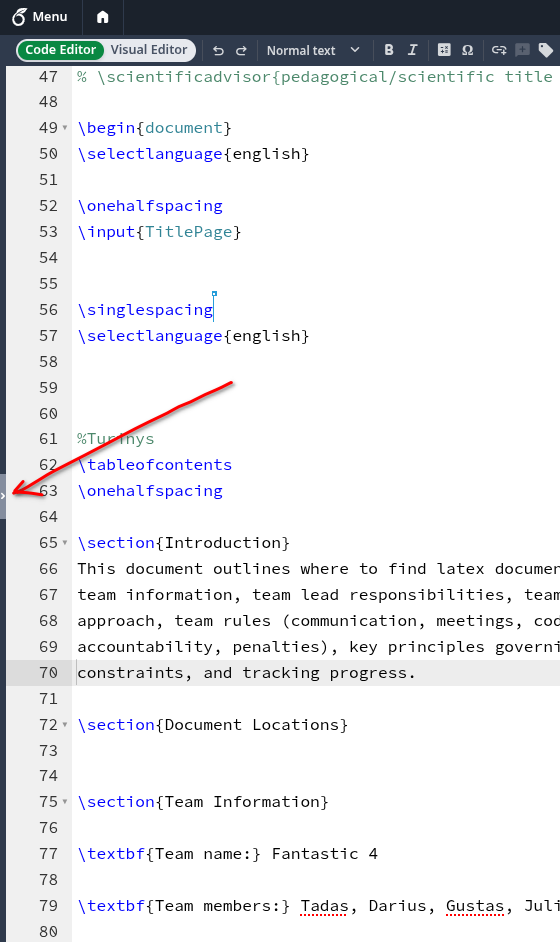
\includegraphics[height=0.45\textheight]{images/find_arrow.png}
    \\[6pt]
    \small\emph{(see first image)}
\end{minipage}\hfill
\begin{minipage}[t]{0.48\linewidth}
    \centering
    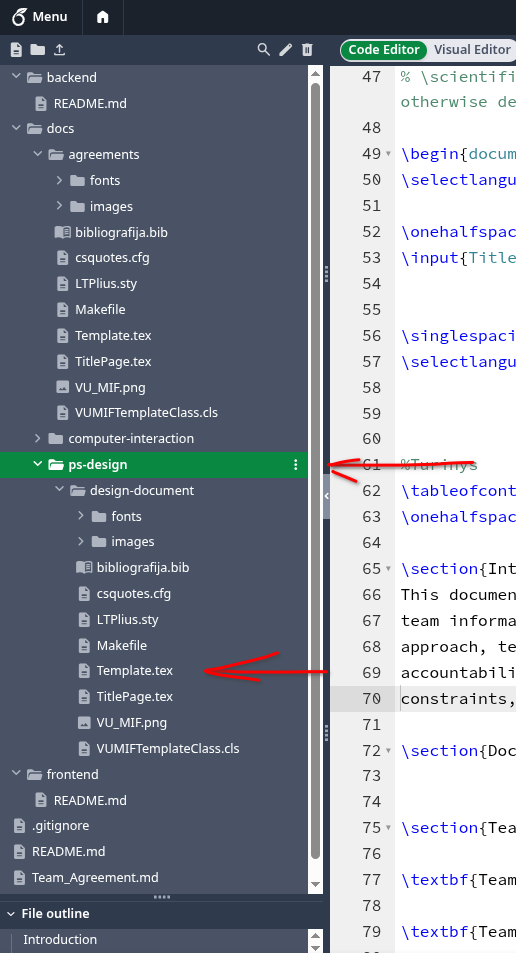
\includegraphics[height=0.45\textheight]{images/find_folder.png}
    \\[6pt]
    \small\emph{(see second image)}
\end{minipage}
\end{figure}

\begin{figure}[H]
\centering
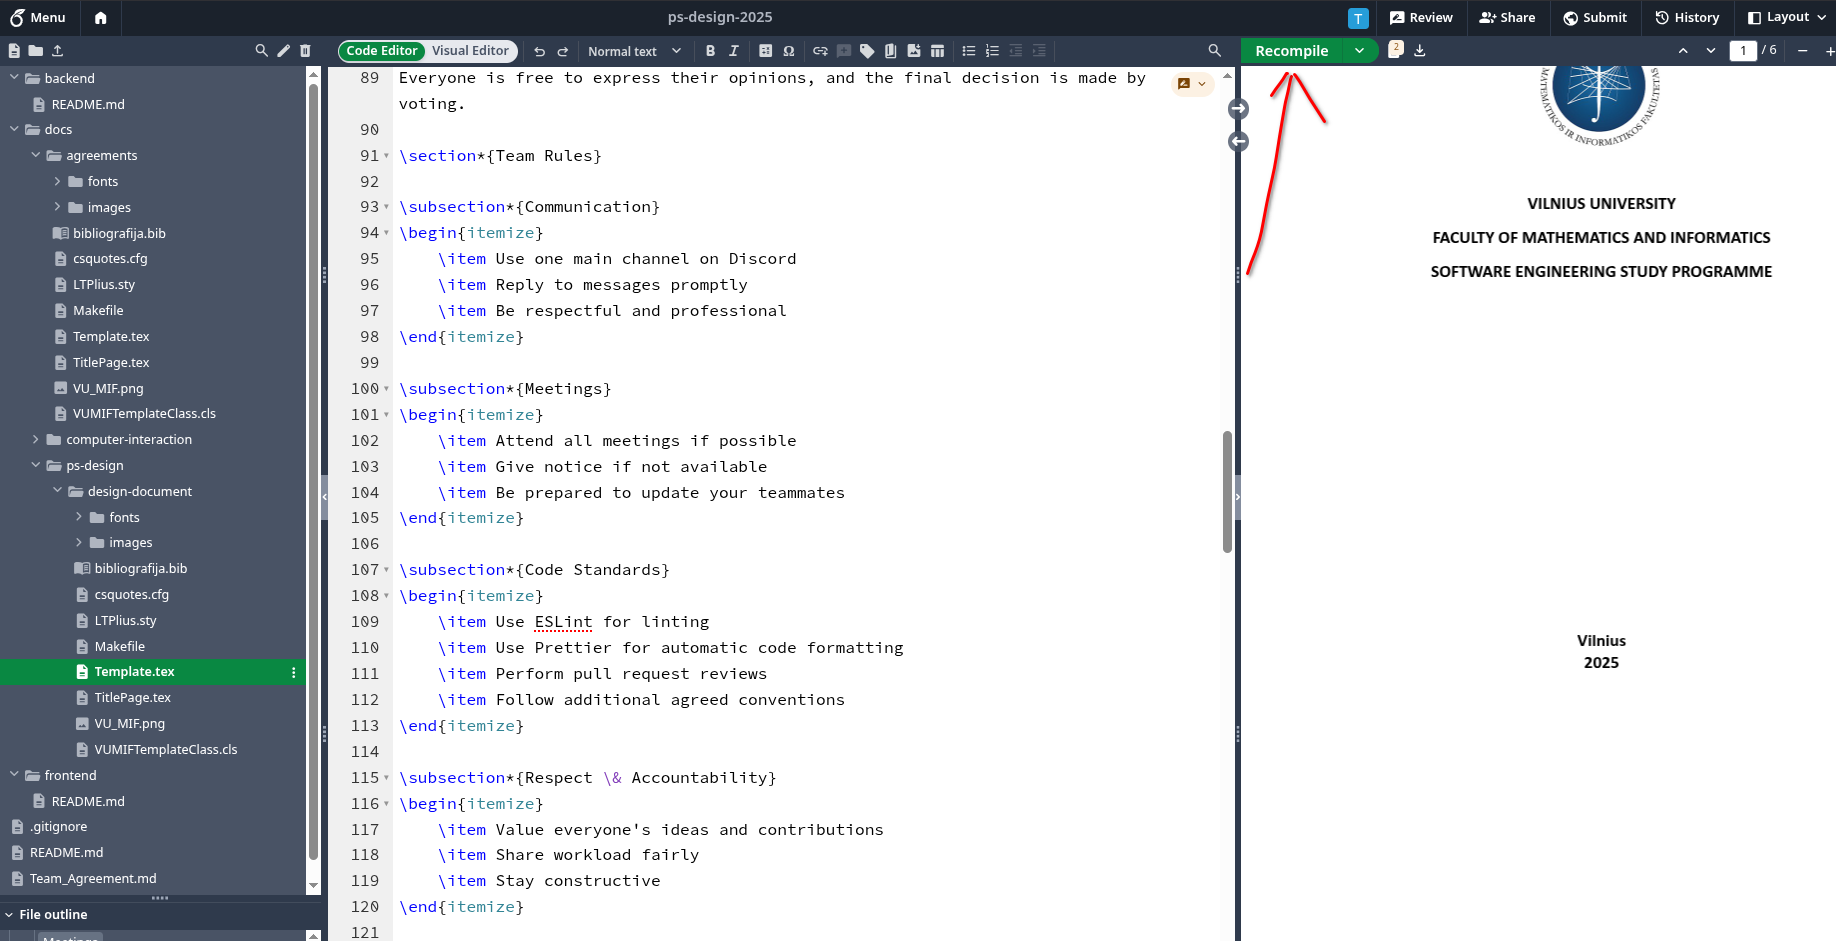
\includegraphics[width=0.9\linewidth]{images/compile.png}
\end{figure}

\noindent To locate the PS Software Design document, first click the small arrow
at the left of the screen to see folder structure (see first image). Then open
the \texttt{ps-design} folder and select \texttt{Template.tex} (see second
image). Finally, compile \texttt{Template.tex} as
shown in the third image to generate the final PDF.

\section{Team Information}

\textbf{Team name:} Fantastic 4 

\textbf{Team members:} Tadas, Darius, Gustas, Julius 

\textbf{Team lead:} Tadas

\textit{Reason: Showed most motivation}

\vspace{1cm}

\begin{table}[H]
\caption{Team lead responsibilities}
\centering
\begin{tabular}{p{0.25\linewidth} p{0.70\linewidth}}
\textbf{Role} & \textbf{Responsibilities} \\
\hline
Team Lead &
\begin{minipage}[t]{\linewidth}
\begin{itemize}
    \item Plan the meetings and consultations with lecturer
    \item Communicate with lecturer
    \item Create a timeline for the tasks that need to be completed
    \item Resolve conflicts
    \item Ensure everyone is putting equal amount of effort
    \item Ensure requirements are met
\end{itemize}
\end{minipage}
\end{tabular}
\label{tab:team-lead-resp}
\end{table}

\vspace{1cm}

\textbf{Ambition:} We aim to achieve a grade of 9 or 10 for our project.

\textbf{Decision-Making Approach:} Everyone is free to express their opinions, and the final decision is made by voting.

\subsection{Team Rules}
We have established the following team rules and guidelines to ensure effective
collaboration and a positive working environment.

\vspace{1cm}

\begin{longtable}{p{0.25\linewidth} p{0.70\linewidth}}
\caption{Team Rules and Guidelines} \\
\textbf{Area} & \textbf{Rules} \\
\hline
\endfirsthead

\multicolumn{2}{c}{{\tablename\ \thetable{} -- Continued from previous page}} \\
\textbf{Area} & \textbf{Rules} \\
\hline
\endhead

\multicolumn{2}{c}{{Continued on next page}} \\
\endfoot

\endlastfoot

Communication &
\begin{minipage}[t]{\linewidth}
\begin{itemize}
    \item Use one main channel on Discord
    \item Reply to messages promptly
    \item Be respectful and professional
\end{itemize}
\end{minipage} \\[6pt]
\multicolumn{2}{@{}c@{}}{\color{gray}\rule{0.95\linewidth}{0.4pt}} \\[6pt]


Meetings &
\begin{minipage}[t]{\linewidth}
\begin{itemize}
    \item Attend all meetings if possible
    \item Give notice if not available
    \item Be prepared to update your teammates
\end{itemize}
\end{minipage} \\[6pt]
\multicolumn{2}{@{}c@{}}{\color{gray}\rule{0.95\linewidth}{0.4pt}} \\[6pt]


Code Standards &
\begin{minipage}[t]{\linewidth}
\begin{itemize}
    \item Use ESLint for linting
    \item Use Prettier for automatic code formatting
    \item Perform pull request reviews
    \item Follow additional agreed conventions
\end{itemize}
\end{minipage} \\[6pt]
\multicolumn{2}{@{}c@{}}{\color{gray}\rule{0.95\linewidth}{0.4pt}} \\[6pt]


Respect \& Accountability &
\begin{minipage}[t]{\linewidth}
\begin{itemize}
    \item Value everyone's ideas and contributions
    \item Share workload fairly
    \item Stay constructive
\end{itemize}
\end{minipage} \\[6pt]
\multicolumn{2}{@{}c@{}}{\color{gray}\rule{0.95\linewidth}{0.4pt}} \\[6pt]


Penalties &
\begin{minipage}[t]{\linewidth}
For missing deadlines, meetings, or work:
\begin{itemize}
    \item Snack tax or beer tax
    \item Extra documentation duty
    \item Bug fix duty
\end{itemize}
\end{minipage} \\[6pt]
\multicolumn{2}{@{}c@{}}{\color{gray}\rule{0.95\linewidth}{0.4pt}} \\[6pt]


Key principles governing work distribution &
\begin{minipage}[t]{\linewidth}
\begin{itemize}
    \item Fairness and balance: Workload should be distributed so no one feels overburdened; try to balance difficulty, effort, and time commitment.
    \item Assign tasks according to strengths and preferences of team members.
    \item Be clear with responsibilities: Each task should have a designated owner and defined expectations.
    \item Track work using GitHub Projects; everyone should see what others are working on and provide regular progress updates.
    \item Avoid tasks that block other tasks; strive for parallel work whenever possible.
    \item Members are responsible for their assigned work, but must communicate and seek help if falling behind.
    \item Be willing to help each other; documentation and communication should allow someone else to pick up a task in progress.
\end{itemize}
\end{minipage} \\[6pt]
\multicolumn{2}{@{}c@{}}{\color{gray}\rule{0.95\linewidth}{0.4pt}} \\[6pt]


Capacity Constraints &
\begin{minipage}[t]{\linewidth}
\begin{itemize}
    \item Each member reports weekly availability so tasks can be planned realistically.
    \item Hold a weekly sync on [FILL IN], plus short check-ins as needed.
    \item Track capacity: record planned hours versus actual hours spent.
    \item If a member cannot meet their capacity, they must inform the team promptly.
\end{itemize}
\end{minipage} \\[6pt]
\multicolumn{2}{@{}c@{}}{\color{gray}\rule{0.95\linewidth}{0.4pt}} \\[6pt]


Tracking Progress &
\begin{minipage}[t]{\linewidth}
\begin{itemize}
    \item Use GitHub Projects to manage tasks and milestones
    \item Hold weekly meetings(Monday evenings) to review progress and plan next week.
\end{itemize}
\end{minipage} \\
\end{longtable}

\subsubsection{Document comments}
Use the comment boxes below to communicate intent, assign action items, and keep track of unresolved issues. Always include who is responsible and, when relevant, a target date.

Best practices:
\begin{itemize}
    \item Short, actionable messages: what, who, when.
    \item Keep context: reference section, figure, or line numbers if needed.
    \item Resolve or delete comments when the item is complete.
    \item Prefer suggestions for non-blocking feedback; use warnings for critical fixes.
\end{itemize}

Examples:
\warningcomment{This is a warning comment. Use it to highlight critical issues that need immediate attention.}
\yellowcomment{This is a yellow comment. Use it for general comments or suggestions.}
\todocomment{This is a to-do comment. Use it to list tasks that need to be completed.}
\noticecomment{This is a notice comment. Use it to provide important information or reminders.}
\goodcomment{This is a good comment. Use it to highlight well-done sections or practices.}
\suggestioncomment{This is a suggestion comment. Use it to propose ideas or improvements.}




\end{document}
